iffalse
\let\negmedspace\undefined
\let\negthickspace\undefined
\documentclass[journal,12pt,twocolumn]{IEEEtran}
\usepackage{cite}
\usepackage{amsmath,amssymb,amsfonts}
\usepackage{graphicx}
\usepackage{textcomp}
\usepackage{xcolor}
\usepackage{txfonts}
\usepackage{listings}
\usepackage{enumitem}
\usepackage{mathtools}
\usepackage{gensymb}
\usepackage{comment}
\usepackage[breaklinks=true]{hyperref}
\usepackage{tkz-euclide} 
\usepackage{listings}
\usepackage{gvv}                                        
\def\inputGnumericTable{}                                 
\usepackage[latin1]{inputenc}                                
\usepackage{color}                                            
\usepackage{array}                                            
\usepackage{longtable}                                       
\usepackage{calc}                                             
\usepackage{multirow}                                         
\usepackage{hhline}                                           
\usepackage{ifthen}                                           
\usepackage{lscape}
\usepackage[export]{adjustbox}

\newtheorem{theorem}{Theorem}[section]
\newtheorem{problem}{Problem}
\newtheorem{proposition}{Proposition}[section]
\newtheorem{lemma}{Lemma}[section]
\newtheorem{corollary}[theorem]{Corollary}
\newtheorem{example}{Example}[section]
\newtheorem{definition}[problem]{Definition}
\newcommand{\BEQA}{\begin{eqnarray}}
\newcommand{\EEQA}{\end{eqnarray}}
\newcommand{\define}{\stackrel{\triangle}{=}}
\newtheorem{rem}{Remark}

\begin{document}
\parindent 0px
\bibliographystyle{IEEEtran}

\vspace{3cm}

\title{}
\author{EE23BTECH11208 - Manohar K$^{*}$
}
\maketitle
\newpage
\bigskip

% \renewcommand{\thefigure}{\theenumi}
% \renewcommand{\thetable}{\theenumi}

\section*{Exercise 9.2}

\noindent \textbf{14.} \hspace{2pt} Insert five numbers between 8 and 26 such that the resulting sequence is an A.P. and obtain the Z-transform of the sequence.

\noindent \textbf{Solution}:
\fi
\noindent
Given,
\begin{table}[h]
    \centering
    
  \begin{tabular}{|c|c|c|}
    \hline
    \textbf{symbol} & \textbf{value} & \textbf{description} \\
    \hline
    $x(0)$ & $8$ & first term of the series \\
    \hline
    $x(6)$ & $26$ & last term of the series \\
    \hline
    $N$ & $2+5=7$ & number terms in the series \\
    \hline
  \end{tabular}
 

    \caption{Parameters}
    \label{tab: 11.9.2.14.1}
\end{table}
\begin{align}
	d&=\frac{x\brak{6} - x\brak{0}}{N-1},\\
    &=3\\
	x\brak{n}&=[x\brak{0}+nd] u\brak{n}
\end{align}\\	
the A.P. sequence is:\\
\begin{align}
8,11,14,17,20,23,26
\end{align}\\
using eq \eqref{eq:apz},
\begin{align}
    \implies X\brak{z}&=\frac{8}{1-z^{-1}} + \frac{3 z^{-1}}{(1-z^{-1})^2} &\cbrak{ROC : z \neq 1}
\end{align}
\begin{figure}[ht]
\centering
   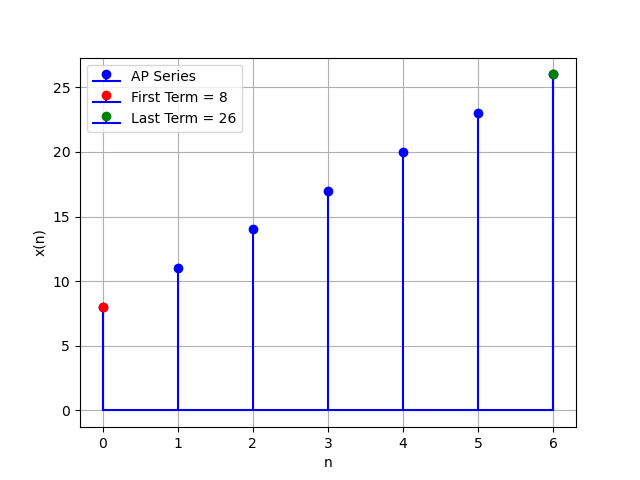
\includegraphics[width=1\linewidth]{figs/plot1.png}
   \caption{Plot of x(n) vs n}
   \hfill\label{fig: 11.9.2.14}
\end{figure}
